\documentclass[11pt,a4paper]{article}
\usepackage[margin=2.5cm]{geometry}
\usepackage{amsmath,amssymb,amsthm}
\usepackage{booktabs}
\usepackage{graphicx}
\usepackage[hidelinks]{hyperref}
\usepackage{siunitx}

\newtheorem{proposition}{Proposition}
\graphicspath{{../results/}}

\title{Ruin, Drawdowns and the Kelly Criterion\\[0.3em]
\large Pass probabilities under prop-firm loss limits, and optimal stakes when the edge is uncertain}
\author{Krish Mod Patel}
\date{30 October 2026}

\begin{document}
\maketitle

\begin{abstract}
A trader taking a funded-account (``prop-firm'') challenge must reach a profit target
before breaching an overall loss limit and a daily loss limit. I derive the classical
gambler's-ruin probability and expected duration by solving a linear recurrence, extend
the model to unequal wins and losses and to a daily limit with an absorbing Markov chain,
and confirm every result by Monte Carlo simulation. I then derive the Kelly stake, which
maximises long-run growth when profits compound, and show how uncertainty about the win
rate changes the answer. Using a personal record of 5 wins in 12 trades with an average
win 2.28 times the average loss, the pass probability at 1\% risk per trade is 96\% if
that record reflects the true edge, but ranges from 2\% to almost 100\% across the 95\%
interval for the true win rate. Twelve trades cannot tell which.
\end{abstract}

\noindent\textit{Note on authorship.} The derivations, code and text of this first
version were produced by an AI assistant (Claude) at my request, checked by running the
code and its tests, and reviewed by a second, separate AI review pass. The input record
is my own. I am working through the derivations to reproduce them independently; the
repository's development log records what was done, by whom and when.

\section{Model}

Each trade wins with probability $p$ and loses with probability $q = 1-p$,
independently. A loss costs a fixed fraction $r$ of the \emph{initial} balance (the
\emph{risk per trade}); a win pays $b r$, where $b$ is the payoff ratio (average win
divided by average loss). Profit and loss (P\&L) is measured as a fraction of the initial
balance. The account \emph{passes} when P\&L reaches the target $T$ and \emph{fails} when
it reaches $-L$, or when the P\&L of a single day reaches $-L_d$ (measured from the
balance at the start of the day). Touching a limit counts as reaching it. The trader
makes $k$ trades a day. Throughout, $T = L = 10\%$, $L_d = 5\%$ and $k = 3$, typical of
a first-phase challenge.

The expected P\&L per trade, in units of $r$, is the \emph{expectancy}
\[
  E = p b - q,
\]
and the break-even win rate is $p = 1/(1+b)$; for $b = 2.28$ it is $30.5\%$.

\section{Equal wins and losses: the gambler's ruin}

Take $b = 1$ and no daily limit. Measure P\&L in steps of $r$ and shift it so the loss
limit is $0$: the account starts at $i = L/r$ and passes at $N = (L+T)/r$, both assumed
to be integers.

\begin{proposition}\label{prop:ruin}
Let $P_i$ be the probability of reaching $N$ before $0$ from $i$, and $\rho = q/p$. Then
\[
  P_i =
  \begin{cases}
    \dfrac{1-\rho^{\,i}}{1-\rho^{N}}, & p \neq q,\\[1.2em]
    \dfrac{i}{N}, & p = q.
  \end{cases}
\]
\end{proposition}

\begin{proof}
Condition on the first trade. With probability $p$ the account moves to $i+1$, with
probability $q$ to $i-1$, and from there the process starts afresh (the Markov
property). Hence
\begin{equation}\label{eq:rec}
  P_i = p\,P_{i+1} + q\,P_{i-1}, \qquad 0 < i < N, \qquad P_0 = 0,\quad P_N = 1.
\end{equation}
This is a linear recurrence with constant coefficients; with its two boundary values
it has exactly one solution, since $P_0$ and $P_1$ determine every later term and
$P_1$ is then fixed by $P_N = 1$. Trying $P_i = \lambda^i$ gives the
characteristic equation $p\lambda^2 - \lambda + q = 0$, whose roots are
\[
  \lambda = \frac{1 \pm \sqrt{1-4pq}}{2p} = \frac{1 \pm |p-q|}{2p},
\]
because $1 - 4pq = (p+q)^2 - 4pq = (p-q)^2$. So the roots are $1$ and $q/p = \rho$.

If $p \neq q$ the roots differ and the general solution is $P_i = A + B\rho^{\,i}$. The
boundary conditions give $A + B = 0$ and $A + B\rho^{N} = 1$, so $B = -1/(1-\rho^N)$ and
$A = 1/(1-\rho^N)$, which is the first case.

If $p = q = \tfrac12$ the root $1$ is repeated and the general solution is
$P_i = A + B i$; the boundaries give $A = 0$ and $B = 1/N$.
\end{proof}

\begin{proposition}\label{prop:duration}
The expected number of trades until the account passes or fails is
\[
  D_i =
  \begin{cases}
    \dfrac{i - N P_i}{q - p}, & p \neq q,\\[1.2em]
    i(N-i), & p = q.
  \end{cases}
\]
\end{proposition}

\begin{proof}
The game ends in finite expected time: in every block of $N$ trades, $N$ straight
wins end it, which has probability $p^N > 0$, so the duration is at most a geometric
number of blocks. Conditioning on the first trade again, and counting that trade,
\[
  D_i = 1 + p\,D_{i+1} + q\,D_{i-1}, \qquad D_0 = D_N = 0.
\]
The homogeneous part is the recurrence~\eqref{eq:rec}, with solutions $A + B\rho^{\,i}$.
For a particular solution of the full equation try $D_i = c\,i$: then
$c\,i = 1 + p\,c(i+1) + q\,c(i-1) = 1 + c\,i + c(p-q)$, so $c = 1/(q-p)$. Therefore
$D_i = i/(q-p) + A + B\rho^{\,i}$. The boundary conditions give $A = -B$ and
$B(1-\rho^N) = N/(q-p)$, so
\[
  D_i = \frac{i}{q-p} - \frac{N}{q-p}\cdot\frac{1-\rho^{\,i}}{1-\rho^N}
      = \frac{i - N P_i}{q-p}.
\]
When $p = q$, the particular solution is instead $D_i = -i^2$ (check:
$-i^2 = 1 - \tfrac12(i+1)^2 - \tfrac12(i-1)^2 = -i^2$), and the boundaries give
$D_i = i(N-i)$.
\end{proof}

For $r = 1\%$ the challenge is $i = 10$, $N = 20$. A fair game ($p = \tfrac12$) passes
with probability $\tfrac12$ after $100$ trades on average. A 5-point edge ($p = 0.55$)
raises this to $88.1\%$ after $76.3$ trades; a 5-point deficit ($p = 0.45$) lowers it to
$11.9\%$.

\section{Unequal payoffs and a daily limit: an absorbing Markov chain}

With $b \neq 1$ the recurrence has unequal steps, and the daily limit makes the outcome
depend on the order of trades within a day, so I use a Markov chain instead.

\paragraph{States.} Replace $b$ by the nearest fraction $w/m$ with denominator at most
$50$ (for $b = 2.28$ this is exact: $57/25$) and count P\&L in units $u = r/m$. A loss is
then $-m$ units and a win $+w$ units, so every reachable P\&L is a whole number of units.
The state is the P\&L at the start of a day, between the two limits.

\paragraph{Transitions.} For each start state, list all $2^k$ win/loss sequences of a
day, each with probability $p^{\text{wins}} q^{\text{losses}}$, and follow the P\&L trade
by trade. A sequence is \emph{absorbed} as soon as the P\&L reaches the target (pass),
the overall limit (fail) or the daily limit relative to the day's start (fail);
otherwise it ends the day in a new state. This gives a matrix $Q$ of transitions between
non-absorbed states and, for each outcome $o$, a vector $R_o$ of one-day absorption
probabilities.

\paragraph{Absorption.} Let $h_o(s)$ be the probability that an account starting the day
in state $s$ eventually ends in outcome $o$. Conditioning on the first day, exactly as in
Proposition~\ref{prop:ruin},
\[
  h_o = R_o + Q\,h_o \quad\Longleftrightarrow\quad (I - Q)\,h_o = R_o,
\]
and the expected number of days $t$ satisfies $(I-Q)\,t = \mathbf{1}$. The matrix
$M = (I-Q)^{-1} = I + Q + Q^2 + \cdots$ is the \emph{fundamental matrix} of the chain
(Kemeny and Snell, 1960): $M_{ij}$ is the expected number of days spent in state $j$
starting from $i$. It exists because absorption is reachable from every state (a run of
wins always passes), so $Q^n \to 0$. The one exception is a rule that forbids every
trade, which the code detects and reports. In practice the sparse
linear systems are solved directly rather than inverting $Q$. Probabilities within a
time limit come from multiplying the start distribution by $Q$ once per day.

\paragraph{Validation.} With $b = 1$, $k = 1$ and no daily limit, the chain reproduces
Propositions~\ref{prop:ruin} and~\ref{prop:duration} to at least six decimal places for
every case tested, and a Monte Carlo simulation of $200{,}000$ accounts per case, which
uses the payoff as given rather than a lattice, agrees within sampling error
(Table~\ref{tab:validation}).

\begin{table}[h]
\centering
\caption{Equal wins and losses, target and loss limit both 10\%. Selected rows; all
eight are in the repository.}
\label{tab:validation}
\begin{tabular}{rrcccrr}
\toprule
$r$ & $p$ & Formula & Chain & Simulation (s.e.) & Formula $D$ & Chain $D$\\
\midrule
1\% & 0.40 & 0.017046 & 0.017046 & 0.0169 (0.0003) & 48.30 & 48.30\\
1\% & 0.45 & 0.118501 & 0.118501 & 0.1189 (0.0007) & 76.30 & 76.30\\
1\% & 0.50 & 0.500000 & 0.500000 & 0.5008 (0.0011) & 100.00 & 100.00\\
1\% & 0.55 & 0.881499 & 0.881499 & 0.8811 (0.0007) & 76.30 & 76.30\\
2\% & 0.40 & 0.116364 & 0.116364 & 0.1158 (0.0007) & 19.18 & 19.18\\
2\% & 0.55 & 0.731717 & 0.731717 & 0.7316 (0.0010) & 23.17 & 23.17\\
\bottomrule
\end{tabular}
\end{table}

\section{The challenge with the record's edge}

My own record is $5$ wins in $12$ trades ($p = 41.7\%$) with $b = 2.28$, an expectancy of
$+0.37$ of the amount risked per trade \emph{if} the record is representative.
Table~\ref{tab:challenge} gives the exact outcome probabilities.

\begin{table}[h]
\centering
\caption{Challenge outcomes for $p = 5/12$, $b = 2.28$, three trades a day.}
\label{tab:challenge}
\begin{tabular}{rrrrrr}
\toprule
Risk $r$ & Pass & Fail (overall) & Fail (daily) & Expected days & Pass within 60 days\\
\midrule
0.25\% & 100.0\% & 0.0\% & 0.0\% & 37.5 & 91.6\%\\
0.5\% & 99.8\% & 0.2\% & 0.0\% & 19.3 & 99.2\%\\
1\% & 96.1\% & 3.9\% & 0.0\% & 9.5 & 96.1\%\\
1.5\% & 89.6\% & 10.4\% & 0.0\% & 5.8 & 89.6\%\\
2\% & 53.0\% & 0.0\% & 47.0\% & 2.4 & 53.0\%\\
3\% & 52.6\% & 0.0\% & 47.4\% & 1.4 & 52.6\%\\
5\% & 41.7\% & 0.0\% & 58.3\% & 1.0 & 41.7\%\\
\bottomrule
\end{tabular}
\end{table}

Three features stand out.

\begin{enumerate}
\item \textbf{The daily limit dominates above 1.5\% risk.} Three losses cost $3r$, which
reaches $5\%$ once $r \ge 5/3\% \approx 1.67\%$; of the risks tested, $2\%$ is the first
above that. The pass probability drops from 90\% at $1.5\%$ to 53\% at $2\%$.
At $r = 2\%$ the overall limit can no longer be reached at all: a day with at most two
losses ends at least $-4\% + 4.56\% = +0.56\%$ up, so every day either gains or breaches
the daily limit. A trader who skips any trade whose loss would breach the daily limit
raises the pass probability at $2\%$ risk from 53\% to 83\%.
\item \textbf{With a positive edge, smaller stakes pass more often but take longer.}
Without a time limit, $r = 0.25\%$ passes almost surely but needs 37.5 days on average;
within 60 trading days $r = 0.5\%$ does best of the risks tested (99.2\%). This is the law of large numbers:
more, smaller trades let the positive expectancy dominate the noise.
\item \textbf{With a negative edge the opposite tends to hold.} For $p = 0.25$
(expectancy $-0.18$) the pass probability rises from $0.1\%$ at $r = 0.25\%$ to $25\%$
at $r = 5\%$, though not monotonically (22\% at $1.5\%$, 15\% at $2\%$) because the
daily limit interferes. When the game is unfavourable, fewer and larger bets give the
negative expectancy fewer chances to act. This is consistent with the intuition behind
Dubins and Savage's (1965) ``bold play'', although their theorem concerns a gambler who
may change the stake after every bet, which this fixed-stake model does not allow.
\end{enumerate}

\paragraph{How much the answer depends on the win rate.} Twelve trades give a 95\%
(Wilson) interval for the true win rate of $19.3\%$ to $68.0\%$. Across that interval
the pass probability at $1\%$ risk runs from $2.0\%$ to almost $100\%$
(Figure~\ref{fig:winrate}); even the break-even win rate of 30.5\% lies inside it.
The record cannot tell a near-certain pass from a near-certain failure.

\begin{figure}[h]
\centering
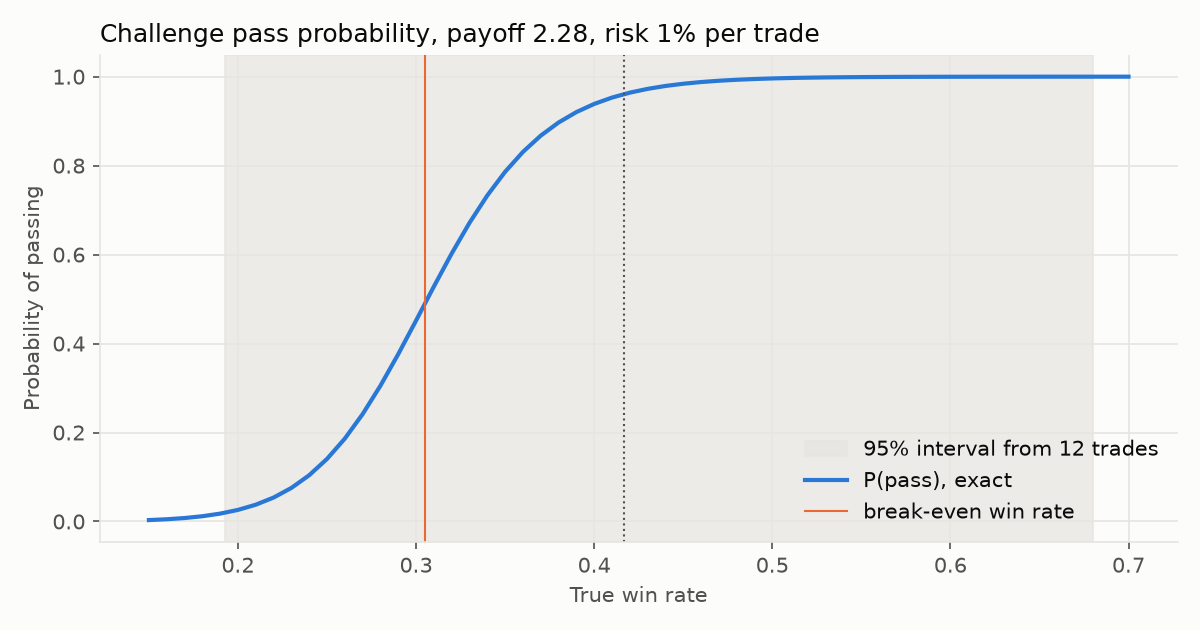
\includegraphics[width=0.85\textwidth]{pass_vs_win_rate.png}
\caption{Exact pass probability against the true win rate, $b = 2.28$, $r = 1\%$.}
\label{fig:winrate}
\end{figure}

\begin{figure}[h]
\centering
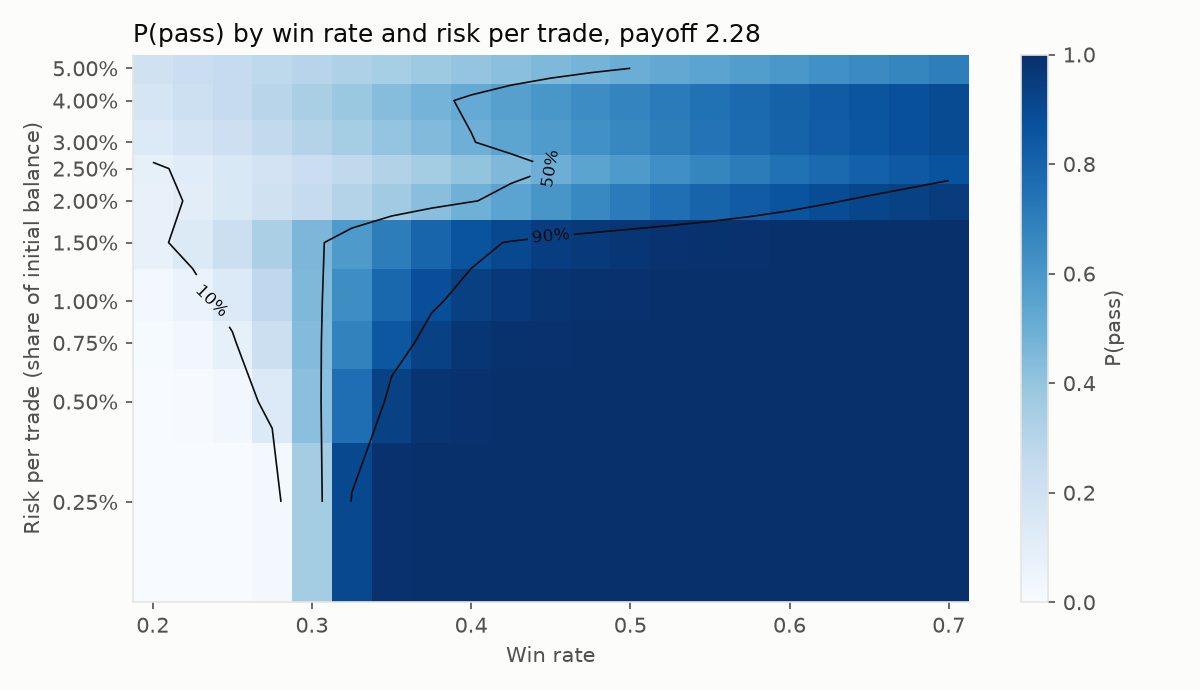
\includegraphics[width=0.85\textwidth]{heatmap_risk.png}
\caption{Pass probability by win rate and risk per trade. The step between 1.5\% and
2\% is the daily limit starting to bind.}
\label{fig:heatmap}
\end{figure}

\section{The Kelly criterion}

The challenge risks a fixed share of the \emph{initial} balance. A trader whose profits
compound instead risks a fraction $f$ of the \emph{current} balance. After $n$ trades with
$W$ wins the balance is multiplied by $(1+bf)^{W}(1-f)^{n-W}$, so the growth rate per
trade is $\tfrac1n\ln\!\big[(1+bf)^{W}(1-f)^{n-W}\big]$, which converges to
\[
  g(f) = p\ln(1+bf) + q\ln(1-f)
\]
by the law of large numbers ($W/n \to p$). Kelly (1956) proposed maximising $g$;
Breiman (1961) proved that the strategy maximising $g$ eventually has more wealth than
any essentially different strategy, with probability one.

\begin{proposition}\label{prop:kelly}
For $0 \le f < 1$, $g$ is strictly concave and is maximised at
\[
  f^* = p - \frac{q}{b},
\]
provided $f^* > 0$. If $f^* \le 0$ (zero or negative expectancy) the best stake is $0$.
\end{proposition}

\begin{proof}
Differentiating,
\[
  g'(f) = \frac{pb}{1+bf} - \frac{q}{1-f}, \qquad
  g''(f) = -\frac{pb^2}{(1+bf)^2} - \frac{q}{(1-f)^2} < 0,
\]
so $g$ is strictly concave and any stationary point is the global maximum. Setting
$g'(f) = 0$: $pb(1-f) = q(1+bf)$, so $pb - q = bf(p+q) = bf$, giving
$f^* = (pb-q)/b = p - q/b$. Since $g'(0) = pb - q$, the function is decreasing from
$f = 0$ when the expectancy is not positive, and the constrained optimum is then $f = 0$.
\end{proof}

For the record, $f^* = 5/12 - (7/12)/2.28 = 16.1\%$ of the balance per trade. Across the
95\% interval for $p$ it runs from $-16.1\%$ (do not trade) to $54.0\%$
(Figure~\ref{fig:kelly}).

\paragraph{Fractional Kelly.} Using $\ln(1+x) \approx x - x^2/2$ for small $f$,
\[
  g(f) \approx f\mu - \tfrac12 f^2 m_2, \qquad \mu = pb - q,\quad m_2 = pb^2 + q,
\]
where $\mu$ and $m_2$ are the mean and second moment of a trade's return per unit
staked. This is a parabola with maximum at $\mu/m_2$, a rough approximation to $f^*$
($0.133$ against the exact $0.161$ for the record). Then
$g(cf^*) \approx g(f^*)\,(2c - c^2)$: half Kelly keeps about 75\% of the growth, and
twice Kelly gives about zero growth. The exact values for the record ($76.2\%$ at half
Kelly, $10.1\%$ at twice Kelly) are close to these approximations even though $f^*$ is
not small.

\paragraph{Drawdowns.} Simulating 20{,}000 paths of 500 trades at the record's edge, the
balance fell at least 50\% below its peak on 24\% of paths at quarter Kelly, 99\% at half
Kelly and 100\% at full Kelly; it fell 80\% below its peak on 0.05\%, 17\% and 99\% of
paths. Full Kelly maximises growth, not comfort.

\begin{figure}[h]
\centering
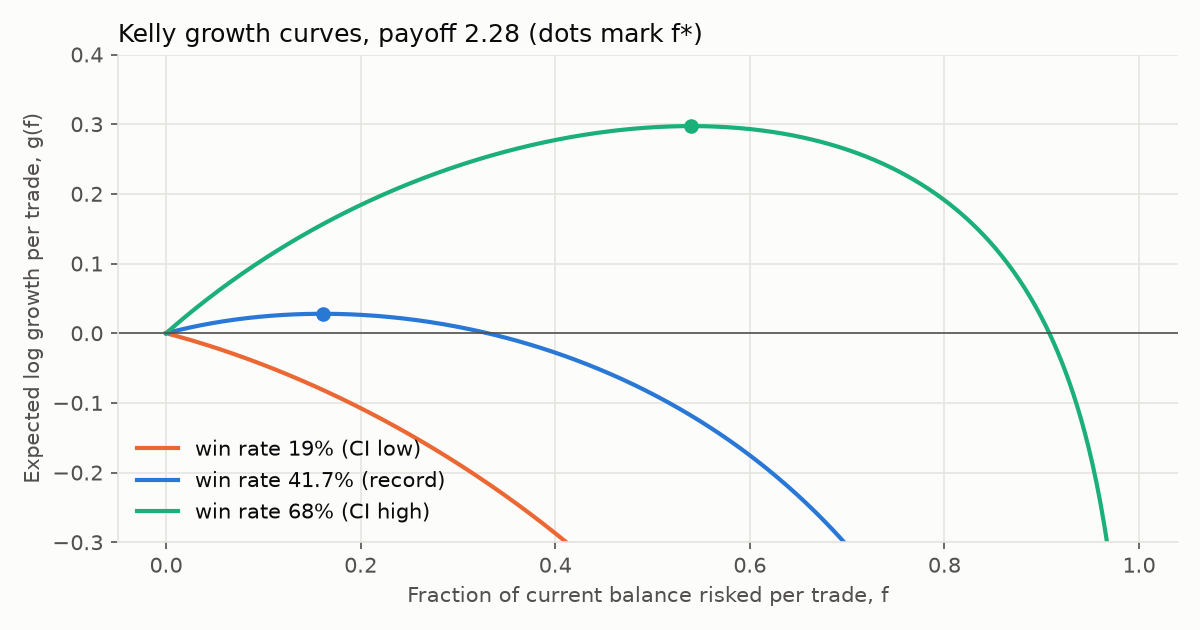
\includegraphics[width=0.85\textwidth]{kelly_growth.png}
\caption{$g(f)$ for $b = 2.28$ at the record's win rate and at both ends of its 95\% interval.}
\label{fig:kelly}
\end{figure}

\section{Kelly with an estimated win rate}

In practice $p$ is unknown. Suppose a trader estimates it from $n$ trades as
$\hat p = W/n$ and then stakes $c\,(\hat p - (1-\hat p)/b)$, set to zero if negative.
Because $W$ is binomial, the expected true growth is an exact finite sum,
\[
  \mathbb{E}[g] = \sum_{w=0}^{n} \binom{n}{w} p^{w} q^{n-w}\;
  g\!\Big(\max\!\big\{0,\; c\,\big(\tfrac{w}{n} - \tfrac{1 - w/n}{b}\big)\big\}\Big),
\]
with $g$ evaluated at the true $p$.

\begin{table}[h]
\centering
\caption{Best multiple $c$ of the estimated Kelly stake, true $p = 5/12$, $b = 2.28$ known.}
\label{tab:estimation}
\begin{tabular}{rcccc}
\toprule
Trades $n$ & Best $c$ & Growth at best $c$ & Growth at $c = 1$ & P(growth $<0$) at $c = 1$\\
\midrule
12 & 0.50 & 55\% & $-9\%$ & 19\%\\
30 & 0.65 & 67\% & 49\% & 7\%\\
100 & 0.85 & 85\% & 82\% & 1\%\\
300 & 0.95 & 94\% & 94\% & 0\%\\
1000 & 1.00 & 98\% & 98\% & 0\%\\
\bottomrule
\end{tabular}
\end{table}

Growth is shown as a share of the growth available to someone who knows $p$. With 12
trades, full Kelly on the estimate gives \emph{negative} expected growth. In 19\% of
samples (7 or more wins out of 12) the estimated stake is at least 40\%, more than
twice $f^*$, where the true growth is negative; because $g$ is concave and falls
steeply beyond $f^*$, those over-bets cost more than the under-bets in other samples
gain. Betting half the estimated stake recovers 55\% of the attainable growth. By 100
trades the penalty for full Kelly is small (82\% of the attainable growth against 85\%
at the best multiple), and by 1{,}000 it disappears.

All stakes in this calculation are capped at $99\%$. Without the cap, full Kelly would
stake everything after a sample of all wins ($\hat p = 1$), an event of probability
$p^n > 0$, and the expected growth would be $-\infty$ for every finite $n$. This calculation also
treats $b$ as known; in reality it is estimated from the same few trades, which makes
the case for a fraction of Kelly stronger still.

A subtle point: if instead one places a Bayesian prior on $p$ and maximises the
\emph{posterior expected} growth, the answer is simply Kelly at the posterior mean,
because $g$ is linear in $p$. Uncertainty in $p$ alone therefore does not shrink the
Bayes-optimal stake; what makes plugging in a point estimate dangerous is the sampling
error of that estimate together with the asymmetry of $g$.

\section{Limitations}

\begin{itemize}
\item Trades are independent with fixed win and loss sizes. Real outcomes vary in size,
cluster in time, and may depend on market conditions.
\item The record of 12 trades is self-reported and unverified; all numbers that use it
are conditional on it.
\item Prop-firm rules differ. Here the overall limit is static, the daily limit is
measured from the start-of-day balance, losses of exactly the limit count as breaches,
and the account passes the moment the target is reached; some firms use trailing
limits, minimum trading days or equity-based measurement.
\item The Kelly analysis ignores costs, and the drawdown results are simulations with
a fixed horizon.
\end{itemize}

\section*{References}
\begin{itemize}
\item[] Dubins, L.~E. and Savage, L.~J. (1965). \emph{How to Gamble If You Must:
Inequalities for Stochastic Processes}. McGraw-Hill.
\item[] Breiman, L. (1961). Optimal gambling systems for favorable games. In
\emph{Proceedings of the Fourth Berkeley Symposium on Mathematical Statistics and
Probability}, Vol.~1, 65--78.
\item[] Feller, W. (1968). \emph{An Introduction to Probability Theory and Its
Applications}, Vol.~1, 3rd ed., Ch.~XIV. Wiley.
\item[] Kelly, J.~L. (1956). A new interpretation of information rate. \emph{Bell
System Technical Journal} 35(4), 917--926.
\item[] Kemeny, J.~G. and Snell, J.~L. (1960). \emph{Finite Markov Chains}. Van Nostrand.
\item[] MacLean, L.~C., Thorp, E.~O. and Ziemba, W.~T. (eds.) (2011). \emph{The Kelly
Capital Growth Investment Criterion}. World Scientific.
\item[] Thorp, E.~O. (2006). The Kelly criterion in blackjack, sports betting and the
stock market. In \emph{Handbook of Asset and Liability Management}, Vol.~1. Elsevier.
\end{itemize}

\end{document}
